\documentclass[10pt, xcolor={dvipsnames}]{beamer}

\usepackage{listings} % source code
\usepackage{ulem}
\usepackage[utf8]{inputenc}
\usepackage[T1]{fontenc}
\usepackage[english]{babel}
\usepackage{hyperref}
\usetheme{Madrid} %\usetheme{CambridgeUS}

\lstset{escapeinside={<@}{@>}}

\setbeamertemplate{footline}[frame number]
\title{A Reverse Engineering Tool for Static Analysis Which Performs Equational	Reasoning on X86 Assembly Code}
\author{Masther Thesis defence\\\textbf{Marien Bourguignon}}
\institute[UMBC]{Université libre de Bruxelles}
\date{September 5, 2016}

\begin{document}

\maketitle

\begin{frame}
	\frametitle{Defence's Organisation}
	\begin{block}{}
		\begin{enumerate}
			\item Relevance of digital reverse engineering
			\item Presentation of an existing dynamic analysis tool
			\item How to extend the tool to perform static analysis
			\item Drawbacks of the potential new tool
		\end{enumerate}
	\end{block}
\end{frame}

\begin{frame}
	\frametitle{Digital Reverse Engineering}
	\begin{definition}{}
		\alert{Digital reverse engineering} is the process of extracting know-how or knowledge from a digital artefact.
	\end{definition}
	\vfill
	\begin{block}{Use cases}
		\begin{itemize}
			\item Software Engineering
			\begin{itemize}
				\item Compiler
				%\item Interoperability
				\item Detecting design patterns
				\item ...
			\end{itemize}
			\item Information Security
			\begin{itemize}
				\item Malware analysis
				\item Cryptographic algorithms 
				\item ...
			\end{itemize}
		\end{itemize}
	\end{block}
\end{frame}

\begin{frame}
	\frametitle{Issue}
	\begin{exampleblock}{}
		{\large “A need exists for tools that can analyse assembly code, whether from disassembled binaries or from handwritten sources.”}
		\vskip5mm
		\hspace*\fill{\small--- \textbf{Kevin Coogan} and \textbf{Saumya Debray}}
	\end{exampleblock}
\end{frame}

\begin{frame}
	\frametitle{Initial Tool}
	\begin{block}{}
		\begin{itemize}
			\item Presented in \textbf{Equational Reasoning on x86 Assembly Code}
			\item Simplifies the comprehension of assembly traces by clearly showing what happened to every variables
%			\begin{itemize}
%				\item By clearly showing what happened to every variables
%				%\item And so making them more readable
%			\end{itemize}
		\end{itemize}
	\end{block}
	\vfill
	\begin{block}{How does it work?}
		\begin{enumerate}
			\item Translates every instruction into a set of equations
			\item Renames operands and resolves the dependencies between equations
			\item Uses equational reasoning to build and simplify expressions for variables
		\end{enumerate}
	\end{block}
\end{frame}



\begin{frame}
	\frametitle{Simple Example}
	\begin{block}{x86 assembly code}
		0: \textcolor{magenta}{pop eax}\\
		1: \textcolor{blue}{mov al, 10}\\
		2: \textcolor{ForestGreen}{add eax, ebx}\\
	\end{block}
	\vfill
	\begin{block}{Translation}
		$\textcolor{magenta}{eax := ValueAt(MLOC[esp..esp+3])}$\\
		$\textcolor{magenta}{esp := esp + 4}$\\
		$\textcolor{blue}{al := 10}$\\
		%$\textcolor{blue}{eax := (eax\ \&\ 1110)\ |\ al}$\\
		$\textcolor{ForestGreen}{eax := eax + ebx}$\\
		$\textcolor{ForestGreen}{eflags := Flag(eax + ebx)}$
	\end{block}
\end{frame}

\begin{frame}
	\frametitle{Simple Example cont'd}
	\begin{block}{Renaming and handling dependencies}
		$\textcolor{magenta}{eax_0 := ValueAt(MLOC[esp_{cons}..esp_{cons}+3])_{cons}}$\\
		$\textcolor{magenta}{esp_0 := esp_{cons} + 4}$\\
		$\textcolor{blue}{al_1 := 10}$\\
		$\textcolor{blue}{eax_1 := (eax_0\ \&\ 1110)\ |\ al_1}$\\
		$\textcolor{ForestGreen}{eax_2 := eax_1 + ebx_{cons}}$\\
		$\textcolor{ForestGreen}{eflags_2 := Flag(eax_1 + ebx_{cons})}$
	\end{block}
	\vfill
	\begin{block}{Equational reasoning}
		$eax_2 := eax_1 + ebx_{cons}$\\
		$eax_2 := (eax_0\ \&\ 1110)\ |\ al_1 + ebx_{cons}$\\
		$eax_2 := (ValueAt(MLOC[esp_{cons}..esp_{cons}+3])_{cons}\ \&\ 1110)\ |\ 10 + ebx_{cons}$
	\end{block}
\end{frame}

\begin{frame}
	\frametitle{Issues When Extending the Tool for Static Analysis}
	\begin{block}{Branching}
	30: $eax_{30} := 10$\\
	31: $eax_{31} := eax_{30} - 1$\\
	32:	$\textcolor{red}{jnz\ 31}$\\\ \\
	\centering \text{Solved the \underline{static single assignment form}}
	\end{block}
	\vfill
	\begin{block}{Indirect addressing}
		$\textcolor{magenta}{ValueAt(MLOC[esp_{cons}..esp_{cons}+3])_0} := 42$\\
		$\textcolor{ForestGreen}{ValueAt(MLOC[ebp_{cons}..ebp_{cons}+3])_1} := 43$\\
		$eax_2 := eax_{cons} \oplus \textcolor{magenta}{ValueAt(MLOC[esp_{cons}..esp_{cons}+3])_0}$\\\ \\
		\centering \text{Solved with \underline{pointer analysis}}
	\end{block}
\end{frame}

\begin{frame}
	\frametitle{Static Single Assignment Form}
	\begin{block}{}
		\begin{itemize}
			\item It is a property a language can have
			\begin{itemize}
				\item It states that each variable can only be assigned once
				\item The notation presented before is in SSA form
			\end{itemize}
			\item It is widely used by compilers to perform optimisations
			\item It uses $\phi$-functions to handle the redefinitions
		\end{itemize}
	\end{block}
	
	\begin{block}{}
		According to \textit{Andrew W. Appel}, SSA is functional programming
	\end{block}
\end{frame}

%\begin{frame}
%	\frametitle{Control Flow Graph}
%	\begin{exampleblock}{}
%		{\large “A \alert{Control Flow Graph} is a directed graph whose nodes are basic blocks and where edges represent the transfer of control between these blocks.”}
%	\end{exampleblock}
%	\hfill
%	\begin{exampleblock}{}
%		{\large “A \alert{basic block} of code is a sequential listing of code which does not have any \textit{in-branches} other than its entry point and no \textit{out-branches} except its exit point.”}
%	\end{exampleblock}
%\end{frame}

\begin{frame}
	\frametitle{CFG and $\phi$-functions}
	\begin{columns}[T] % align columns
		\begin{column}{.48\textwidth}
			\begin{block}{Before}
				\begin{figure}
					\centering
					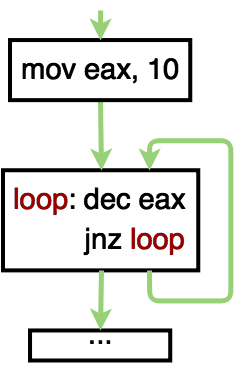
\includegraphics[width = 0.5\textwidth]{simple_cfg.png}
				\end{figure}
			\end{block}
		\end{column}%
		\hfill%
		\begin{column}{.48\textwidth}
			\begin{block}{After}
				\begin{figure}
					\centering
					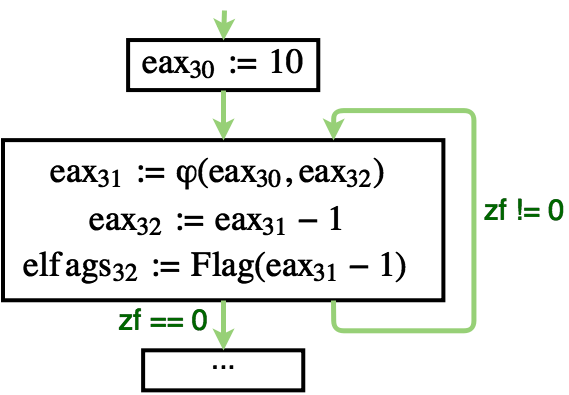
\includegraphics[width = 1\textwidth]{simple_cfg_phi.png}
				\end{figure}
			\end{block}
		\end{column}%
	\end{columns}
\end{frame}



\begin{frame}
	\frametitle{Pointer Analysis}
	\begin{exampleblock}{}
		{\large “\alert{Pointer analysis} is a static code analysis technique which provides information about where pointers may point to.”}
	\end{exampleblock}
	
	\begin{block}{}
		Achieved using the \textbf{value-set analysis} presented by Gogul Balakrishnan et al in \textit{Analyzing Memory Accesses in x86 Executables}.
	\end{block}
	
	\begin{block}{Why the value-set analysis?}
		\begin{itemize}
			\item Does not depend on debugging information
			\item Analyses registers, and also memory locations
			\item Designed to work on x86 assembly
		\end{itemize}
	\end{block}
\end{frame}

%\begin{frame}
%	\frametitle{Value-Set Analysis}
%	\begin{exampleblock}{}
%		{\large “The \alert{value-set analysis} tracks the pointer-valued and integer-valued quantities that a program's data objects can hold, using a set of abstract data objects, called a-locs.”}
%		\vskip5mm
%		\hspace*\fill{\small--- Analyzing Memory Accesses in x86 Executables}
%	\end{exampleblock}
%	
%	\begin{block}{An a-loc can represent the following objects:}
%		\begin{itemize}
%			\item Set of locations between two statically known, adjacent, locations 
%			\begin{itemize}
%				\item Represents global variables
%			\end{itemize}
%			\item Set of locations between two adjacent static stack frame offsets
%			\begin{itemize}
%				\item Represents local variables
%			\end{itemize}
%			\item Registers
%			\item Malloc sites
%		\end{itemize}
%	\end{block}
%\end{frame}

\begin{frame}
	\frametitle{Value-Set Analysis}
	\begin{exampleblock}{}
		{\large “The \alert{value-set analysis} determines an over-approximation of the set of addresses and integer values that each data object can hold at each program point.”}
		\vskip5mm
		\hspace*\fill{\small--- Analyzing Memory Accesses in x86 Executables}
	\end{exampleblock}
	\hfill
	\begin{block}{How does it work?}
		\begin{itemize}
			\item Divides the memory space into memory regions
			\begin{itemize}
				\item One per procedure, one per heap-allocation statement, and a global region
			\end{itemize}
			\item Finds the abstract locations
			\begin{itemize}
				\item An a-loc is a set of locations between two consecutive addresses or offsets
				\item It also encompasses registers
			\end{itemize}
			\item Uses abstract interpretation techniques to over-approximate the values a-locs can take at every program point
		\end{itemize}
	\end{block}
\end{frame}

\begin{frame}
	\frametitle{Example}
	\begin{figure}
		\centering
		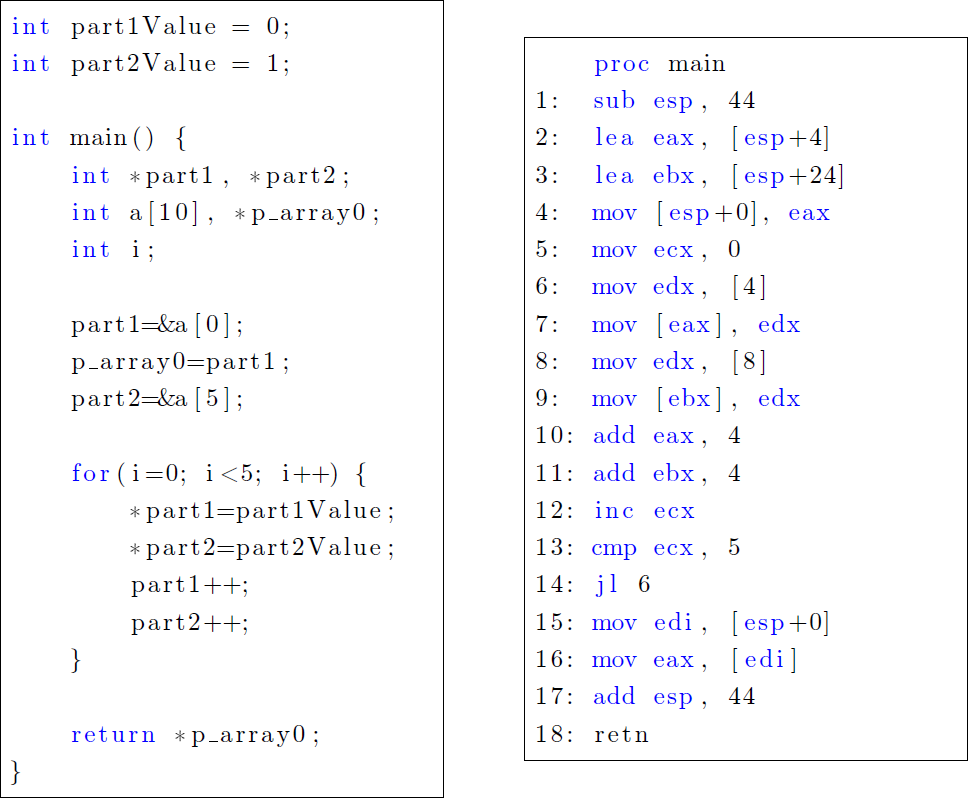
\includegraphics[width = 0.78\textwidth]{vsa_example.png}
	\end{figure}
\end{frame}

\begin{frame}
	\frametitle{Example cont'd}
	\begin{columns}[T] % align columns
		\begin{column}{.48\textwidth}
			\begin{block}{Data layout}
				\begin{figure}
					\centering
					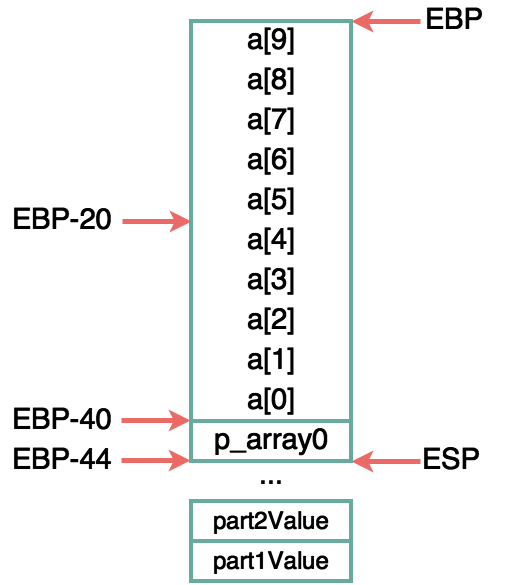
\includegraphics[width = 1\textwidth]{data_layout.png}
				\end{figure}
			\end{block}
		\end{column}%
		\hfill%
		\begin{column}{.48\textwidth}
			\begin{block}{Memory regions}
				\begin{figure}
					\centering
					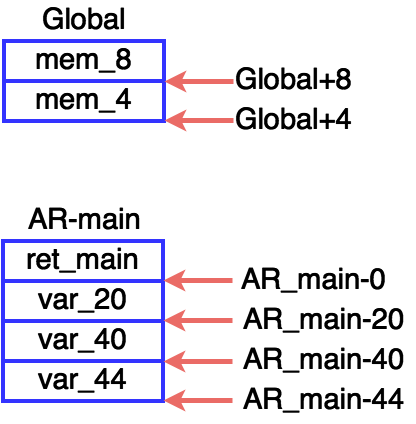
\includegraphics[width = 0.9\textwidth]{memory_region.png}
				\end{figure}
			\end{block}
		\end{column}%
	\end{columns}
\end{frame}

\begin{frame}
	\frametitle{Example cont'd}
	\begin{columns}[T] % align columns
		\begin{column}{.48\textwidth}
			\begin{block}{Assembly}
			\begin{figure}
				\centering
				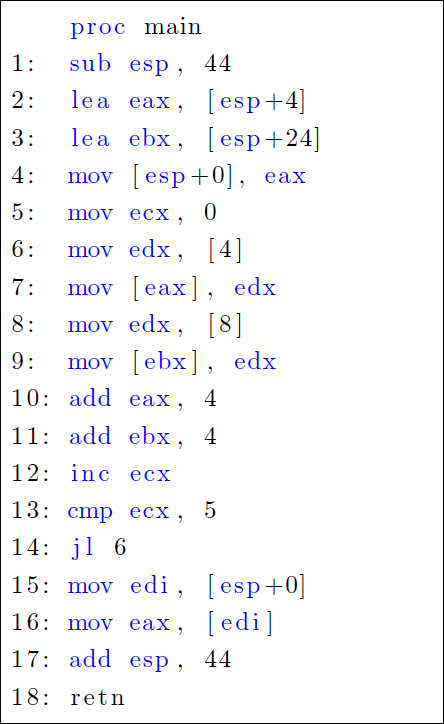
\includegraphics[width = 0.7\textwidth]{vsa_only_assembly.png}
			\end{figure}
			\end{block}
		\end{column}%
		\hfill%
		\begin{column}{.48\textwidth}
			\begin{block}{VSA output for line 7}
				\begin{itemize}
					\item $mem_4 \rightarrow (0, \bot)$
					\item $mem_8 \rightarrow (1, \bot)$
					\item $var_{44} \rightarrow (\bot, -40)$
					\item $ecx \rightarrow (\bot, [0, 4])$
					\item $eax \rightarrow (\bot, 4[0, \infty]-40)$
					\item $ebx \rightarrow (\bot, 4[0, \infty]-20)$
					\item $esp \rightarrow (\bot, -44)$
				\end{itemize}
			\end{block}
		\end{column}%
	\end{columns}
\end{frame}

\begin{frame}[fragile]
	\frametitle{$\chi$-functions}
	\begin{columns}[T] % align columns
		\begin{column}{.48\textwidth}
			\begin{block}{Aliased}
			\begin{lstlisting}[language=C]
<@$ [a]_1 := 42 $@>
<@$ [b]_2 := 43 $@>
<@$ [a]_2 := [b]_2 $@>
			\end{lstlisting}
			\end{block}
		\end{column}%
		\hfill%
		\begin{column}{.48\textwidth}
			\begin{block}{May be aliased}
			\begin{lstlisting}[language=C]
<@$ [a]_1 := 42 $@>
<@$ [b]_2 := 43 $@>
<@$ [a]_2 := \chi([a]_1, [b]_2) $@>
			\end{lstlisting}
			\end{block}
		\end{column}%
	\end{columns}
\end{frame}

\begin{frame}
	\frametitle{Description of the Static Analysis}
	\begin{block}{}
		\begin{enumerate}
			\item Apply the value-set analysis on the binary
			\item Generate the control flow graph of the binary
			\item Translate the instructions to sets of equations, without putting any subscript
			\item Insert the $\phi$-functions using the dominance frontier
			\item Insert the $\chi$-functions using the result from the value-set analysis
			\item Resolve the dependencies by renaming variables and adding equations
			\item Build expressions for the variables of interest using equational reasoning
		\end{enumerate}
	\end{block}
\end{frame}

\begin{frame}
	\frametitle{Drawbacks}
	\begin{block}{Drawbacks}
		\begin{itemize}
			\item The value-set analysis relies on the assumption that the code has been compiled from a high level language
			\item The value-set analysis only provides an approximation of the values variables can take
			\item The $\phi$/$\chi$-functions will decrease the readability of the output
			\item The tool is hard to implement, more so if done from scratch
		\end{itemize}
	\end{block}
\end{frame}

\begin{frame}
	\frametitle{Decrease of Readability}
		\begin{columns}[T] % align columns
			\begin{column}{.42\textwidth}
				\begin{block}{Control flow graph}
					\begin{figure}
						\centering
						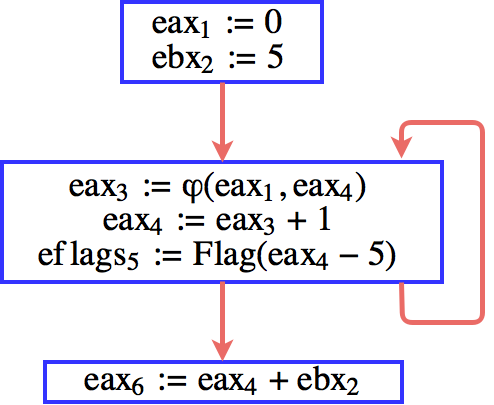
\includegraphics[width = 1\textwidth]{limitation_cfg.png}
					\end{figure}
				\end{block}
			\end{column}%
			\hfill%
			\begin{column}{.54\textwidth}
				\begin{block}{“Readable” expression}
					\begin{enumerate}
						\item $eax_6 := eax_4 + ebx_2$
						\item $eax_6 := eax_3 + 1 + 5$
						\item $eax_6 := \phi(eax_1, eax_4) + 1 + 5$
						\item $eax_6 := \phi(0, eax_3 + 1) + 1 + 5$
						\item $eax_6 := \phi(0, \phi(eax_1, eax_4) + 1) + 1 + 5$
						\item $eax_6 := \phi(0, \phi(0, eax_4) + 1) + 1 + 5$
					\end{enumerate}
				\end{block}
			\end{column}%
		\end{columns}
\end{frame}

\begin{frame}
	\frametitle{Conclusion}
	\begin{block}{}
		\begin{itemize}
			\item The output of the new tool will be far less readable
			\item The value-set analysis relies on assumption about the data layout
			\item One might wonder if a decompiler would not be more appropriate
		\end{itemize}
	\end{block}
\end{frame}

\begin{frame}
	\frametitle{Equational Reasoning}
	\begin{block}{}
		\begin{itemize}
			\item Elementary algebra, but for programs
			\begin{itemize}
				\item Allows to perform substitutions
			\end{itemize}
			\item Only works with purely functional languages
			\begin{itemize}
				\item i.e. languages that are referentially transparent
			\end{itemize}
			%\item Can be used to prove properties of programs
		\end{itemize}
	\end{block}
	\vfill
	\begin{block}{Example in Haskell}
		\textcolor{magenta}{square x} = \textcolor{ForestGreen}{x * x}\\
		pythagoras a b = \textcolor{magenta}{square a} + \textcolor{magenta}{square b}\\
		pythagoras' a b = \textcolor{ForestGreen}{a * a} + \textcolor{ForestGreen}{b * b}
	\end{block}
\end{frame}

\begin{frame}
	\frametitle{Where to Put the $\phi$-Functions}
	\begin{exampleblock}{}
		{\large “The \alert{dominance frontier} of a node X is the set of all nodes Y that are not strictly dominated by X while having at least one successor which is dominated by X.”}
	\end{exampleblock}

	\begin{figure}
		\centering
		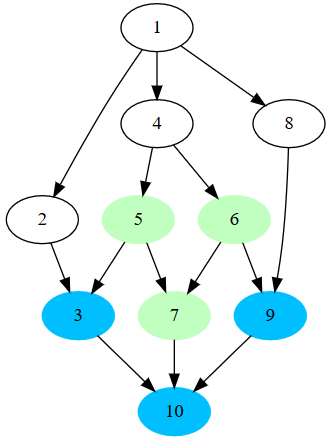
\includegraphics[width = 0.35\textwidth]{graph_dominance_frontier.png}
	\end{figure}
\end{frame}

\begin{frame}
	\frametitle{More on Dependency Resolution}
	\begin{block}{}
		\begin{enumerate}
			\item A source operand is \textbf{fully defined} by a previous destination operand
			\item A source operand is a \textbf{subset} of a previous destination operand
			\item A source operand is defined by a \textbf{subsets of multiple} destination operands
			\item A source operands is defined by multiple destinations operands, while \textbf{none is a subset of the other}
			\item Nothing can be said about an operand
		\end{enumerate}
	\end{block}
\end{frame}

\end{document}